\section{Resultados e discussão dos resultados}\label{sec:resultados}

Nesta sessão serão apresentados os resultados dos experimentos. Abaixo os gráficos de FMR/FNMR e BAcc para cada usuário, em ambos os conjuntos de dados utilizados.


\begin{figure}[H]
    \caption{Magalhães (CMU) - FMR e FNMR}
    \label{fig:Magalhães (CMU) - FMR e FNMR}
    \centering
    \includegraphics[width=\textwidth]{Magalhães (CMU) - FMR e FNMR.png}
\end{figure}
\begin{figure}[H]
    \caption{Magalhães (Keyrecs) - FMR e FNMR}
    \label{fig:Magalhães (Keyrecs) - FMR e FNMR}
    \centering
    \includegraphics[width=\textwidth]{Magalhães (Keyrecs) - FMR e FNMR.png}
\end{figure}
\begin{figure}[H]
    \caption{Magalhães com HPO global (CMU) - FMR e FNMR}
    \label{fig:Magalhães com HPO global (CMU) - FMR e FNMR}
    \centering
    \includegraphics[width=\textwidth]{Magalhães com HPO global (CMU) - FMR e FNMR.png}
\end{figure}
\begin{figure}[H]
    \caption{Magalhães com HPO global (Keyrecs) - FMR e FNMR}
    \label{fig:Magalhães com HPO global (Keyrecs) - FMR e FNMR}
    \centering
    \includegraphics[width=\textwidth]{Magalhães com HPO global (Keyrecs) - FMR e FNMR.png}
\end{figure}
\begin{figure}[H]
    \caption{Magalhães com HPO por usuário (CMU) - FMR e FNMR}
    \label{fig:Magalhães com HPO por usuário (CMU) - FMR e FNMR}
    \centering
    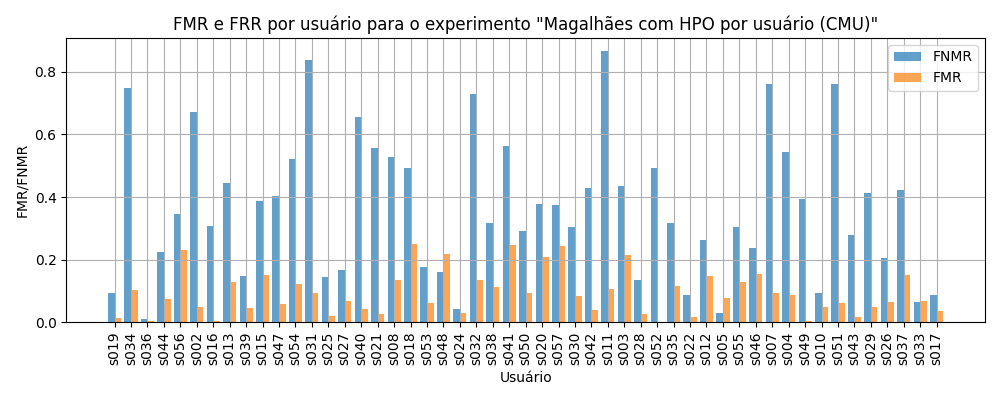
\includegraphics[width=\textwidth]{Magalhães com HPO por usuário (CMU) - FMR e FNMR.png}
\end{figure}
\begin{figure}[H]
    \caption{Magalhães com HPO por usuário (Keyrecs) - FMR e FNMR}
    \label{fig:Magalhães com HPO por usuário (Keyrecs) - FMR e FNMR}
    \centering
    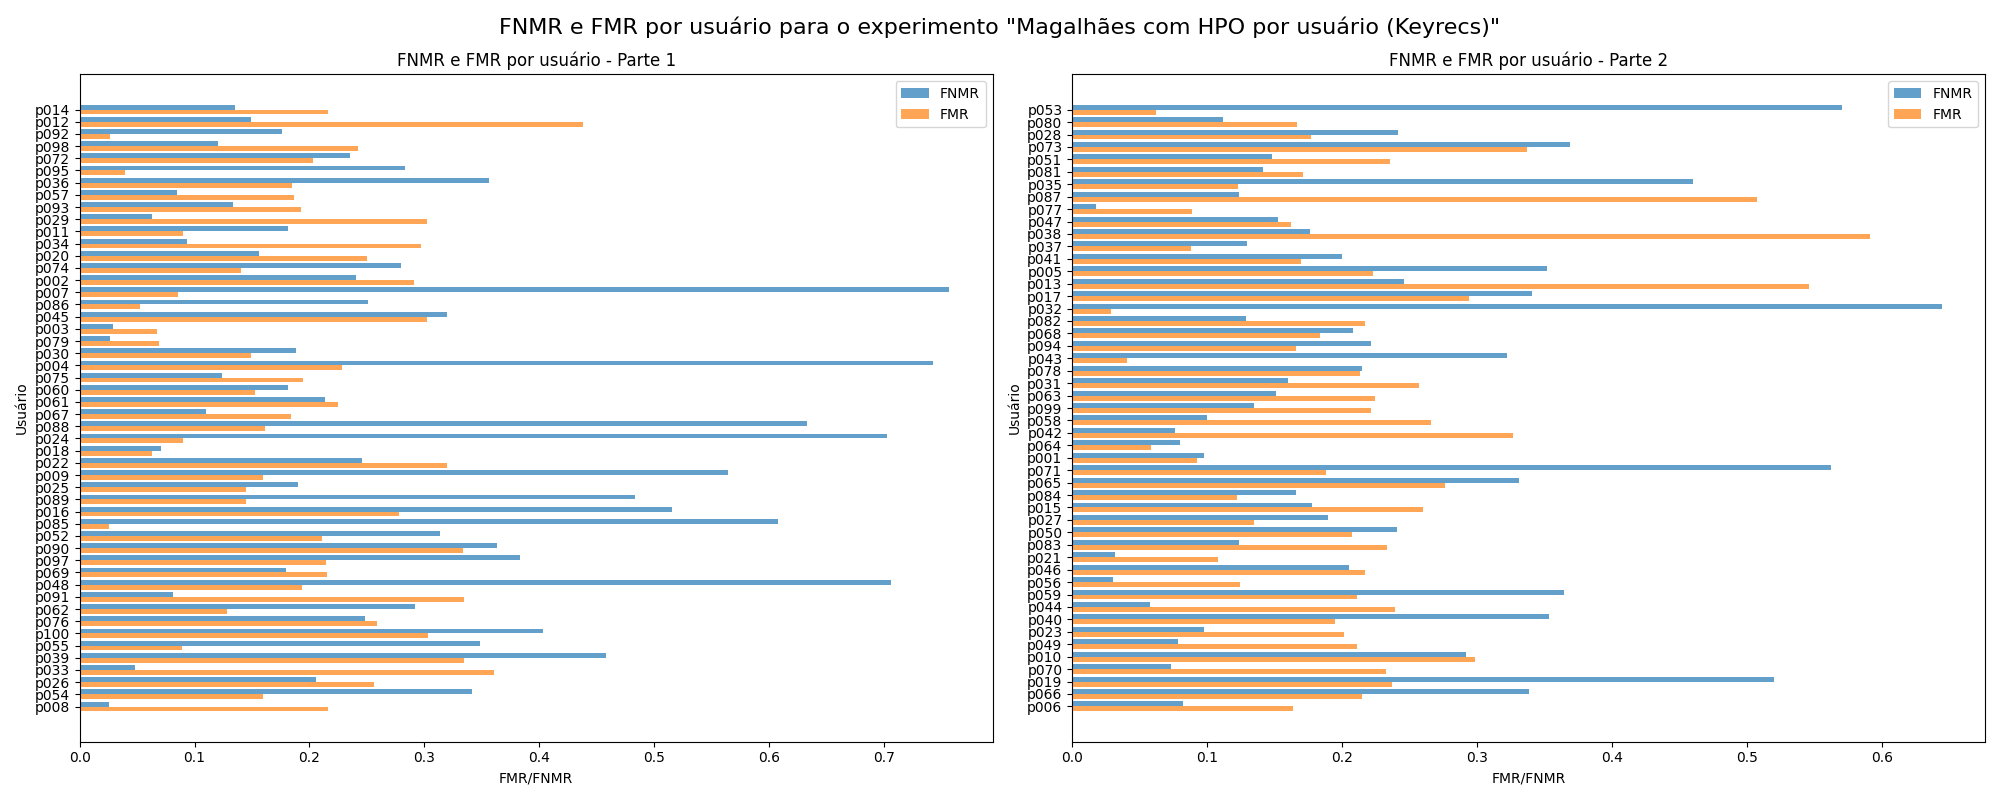
\includegraphics[width=\textwidth]{Magalhães com HPO por usuário (Keyrecs) - FMR e FNMR.png}
\end{figure}
\begin{figure}[H]
    \caption{Random Forest com HPO global (CMU) - FMR e FNMR}
    \label{fig:Random Forest com HPO global (CMU) - FMR e FNMR}
    \centering
    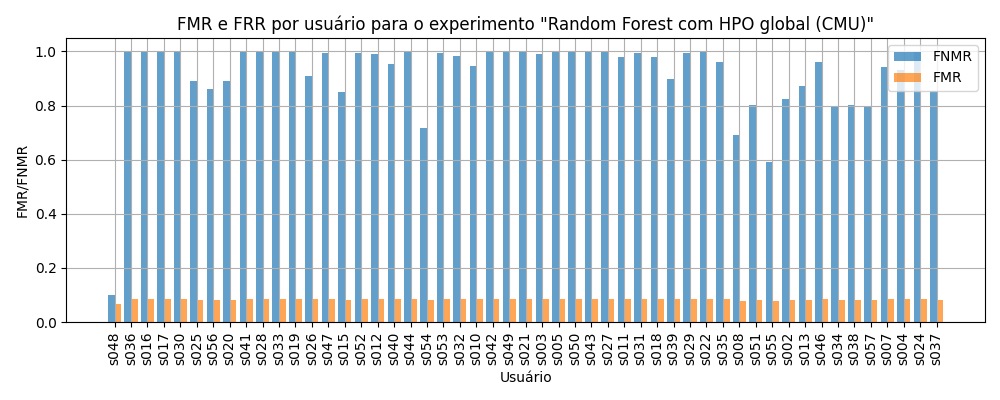
\includegraphics[width=\textwidth]{Random Forest com HPO global (CMU) - FMR e FNMR.png}
\end{figure}
\begin{figure}[H]
    \caption{Random Forest com HPO por usuário (CMU) - FMR e FNMR}
    \label{fig:Random Forest com HPO por usuário (CMU) - FMR e FNMR}
    \centering
    \includegraphics[width=\textwidth]{Random Forest com HPO por usuário (CMU) - FMR e FNMR.png}
\end{figure}
\begin{figure}[H]
    \caption{SVM (CMU) - FMR e FNMR}
    \label{fig:SVM (CMU) - FMR e FNMR}
    \centering
    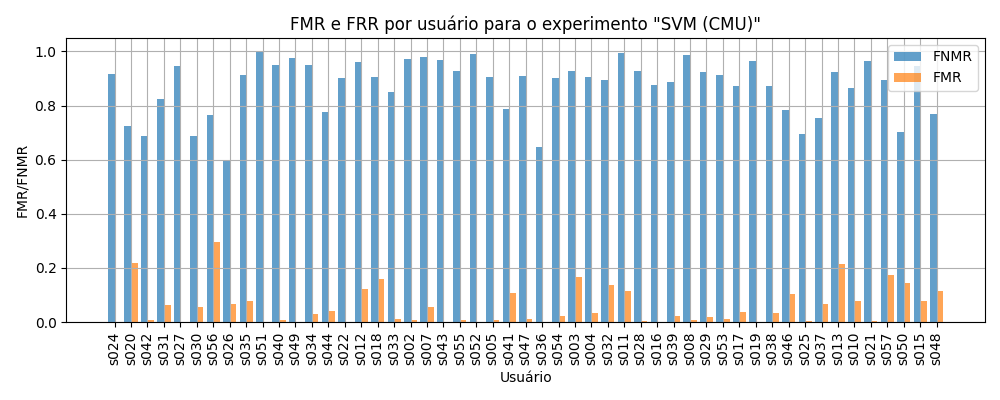
\includegraphics[width=\textwidth]{SVM (CMU) - FMR e FNMR.png}
\end{figure}
\begin{figure}[H]
    \caption{SVM (Keyrecs) - FMR e FNMR}
    \label{fig:SVM (Keyrecs) - FMR e FNMR}
    \centering
    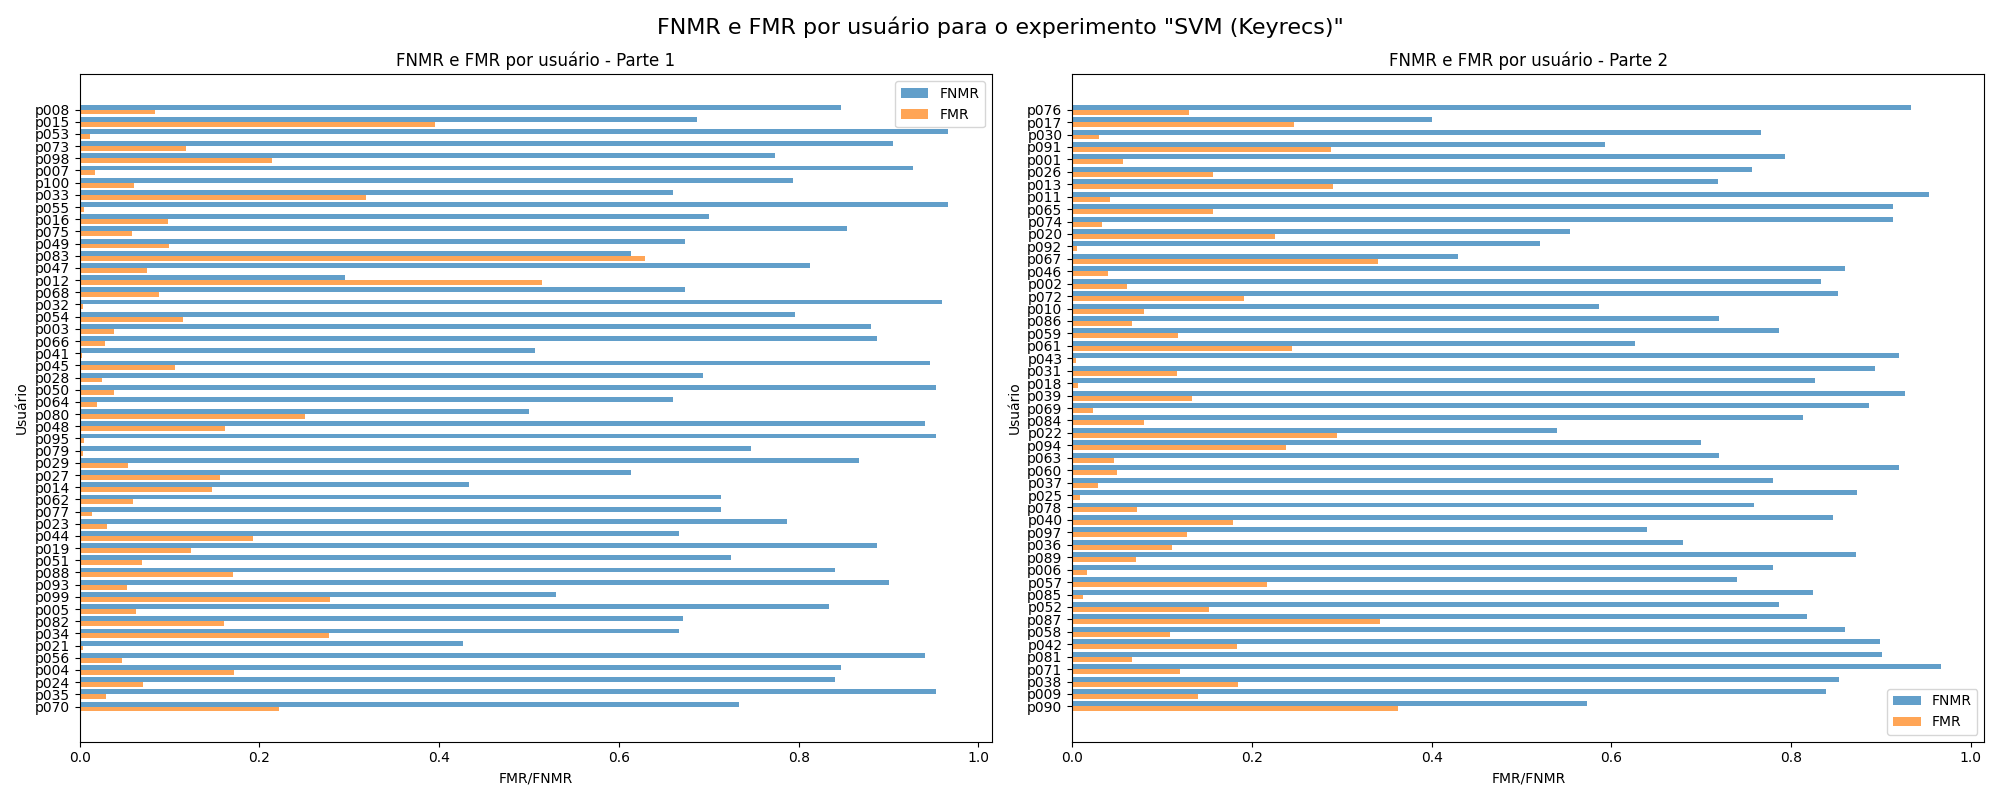
\includegraphics[width=\textwidth]{SVM (Keyrecs) - FMR e FNMR.png}
\end{figure}
\begin{figure}[H]
    \caption{SVM com HPO global (CMU) - FMR e FNMR}
    \label{fig:SVM com HPO global (CMU) - FMR e FNMR}
    \centering
    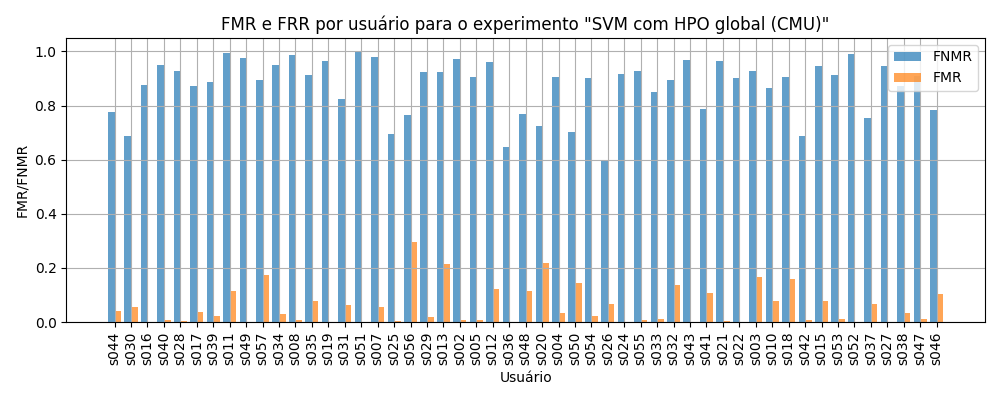
\includegraphics[width=\textwidth]{SVM com HPO global (CMU) - FMR e FNMR.png}
\end{figure}
\begin{figure}[H]
    \caption{SVM com HPO global (Keyrecs) - FMR e FNMR}
    \label{fig:SVM com HPO global (Keyrecs) - FMR e FNMR}
    \centering
    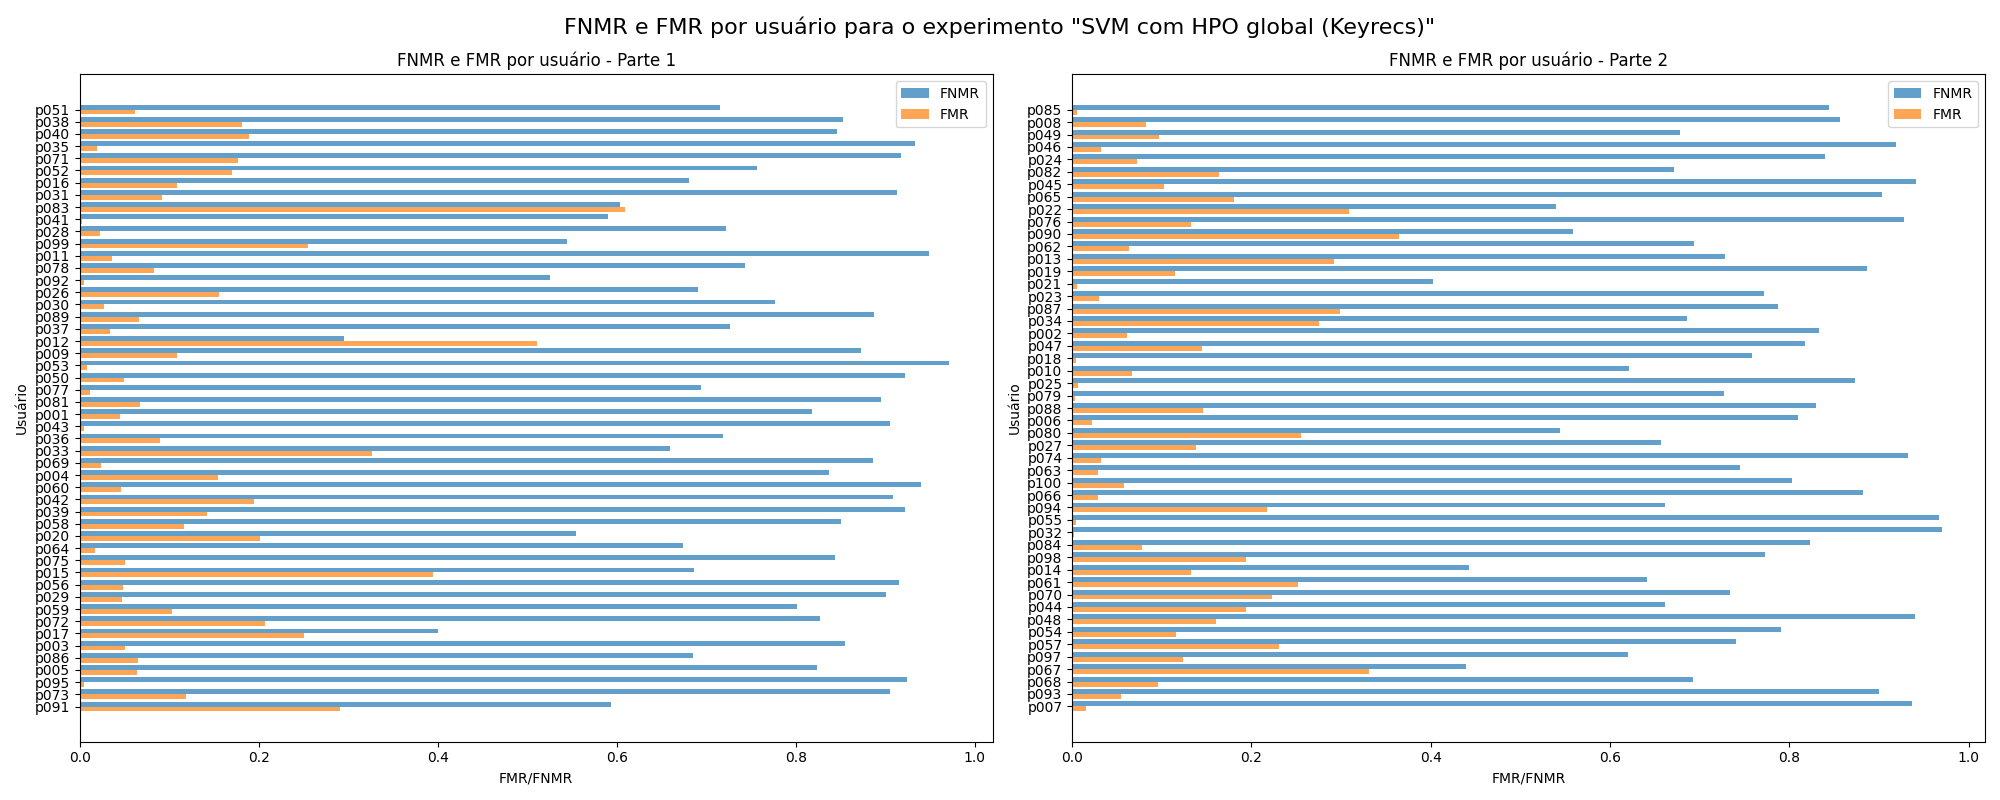
\includegraphics[width=\textwidth]{SVM com HPO global (Keyrecs) - FMR e FNMR.png}
\end{figure}
\begin{figure}[H]
    \caption{SVM com HPO por usuário (CMU) - FMR e FNMR}
    \label{fig:SVM com HPO por usuário (CMU) - FMR e FNMR}
    \centering
    \includegraphics[width=\textwidth]{SVM com HPO por usuário (CMU) - FMR e FNMR.png}
\end{figure}
\begin{figure}[H]
    \caption{SVM com HPO por usuário (Keyrecs) - FMR e FNMR}
    \label{fig:SVM com HPO por usuário (Keyrecs) - FMR e FNMR}
    \centering
    \includegraphics[width=\textwidth]{SVM com HPO por usuário (Keyrecs) - FMR e FNMR.png}
\end{figure}
\begin{figure}[H]
    \caption{Magalhães (CMU) - BAcc}
    \label{fig:Magalhães (CMU) - BAcc}
    \centering
    \includegraphics[width=\textwidth]{Magalhães (CMU) - BAcc.png}
\end{figure}
\begin{figure}[H]
    \caption{Magalhães (Keyrecs) - BAcc}
    \label{fig:Magalhães (Keyrecs) - BAcc}
    \centering
    \includegraphics[width=\textwidth]{Magalhães (Keyrecs) - BAcc.png}
\end{figure}
\begin{figure}[H]
    \caption{Magalhães com HPO global (CMU) - BAcc}
    \label{fig:Magalhães com HPO global (CMU) - BAcc}
    \centering
    \includegraphics[width=\textwidth]{Magalhães com HPO global (CMU) - BAcc.png}
\end{figure}
\begin{figure}[H]
    \caption{Magalhães com HPO global (Keyrecs) - BAcc}
    \label{fig:Magalhães com HPO global (Keyrecs) - BAcc}
    \centering
    \includegraphics[width=\textwidth]{Magalhães com HPO global (Keyrecs) - BAcc.png}
\end{figure}
\begin{figure}[H]
    \caption{Magalhães com HPO por usuário (CMU) - BAcc}
    \label{fig:Magalhães com HPO por usuário (CMU) - BAcc}
    \centering
    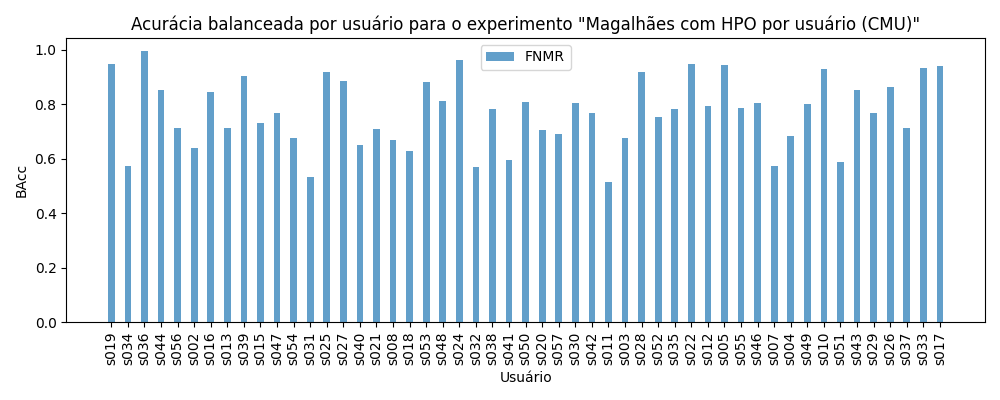
\includegraphics[width=\textwidth]{Magalhães com HPO por usuário (CMU) - BAcc.png}
\end{figure}
\begin{figure}[H]
    \caption{Magalhães com HPO por usuário (Keyrecs) - BAcc}
    \label{fig:Magalhães com HPO por usuário (Keyrecs) - BAcc}
    \centering
    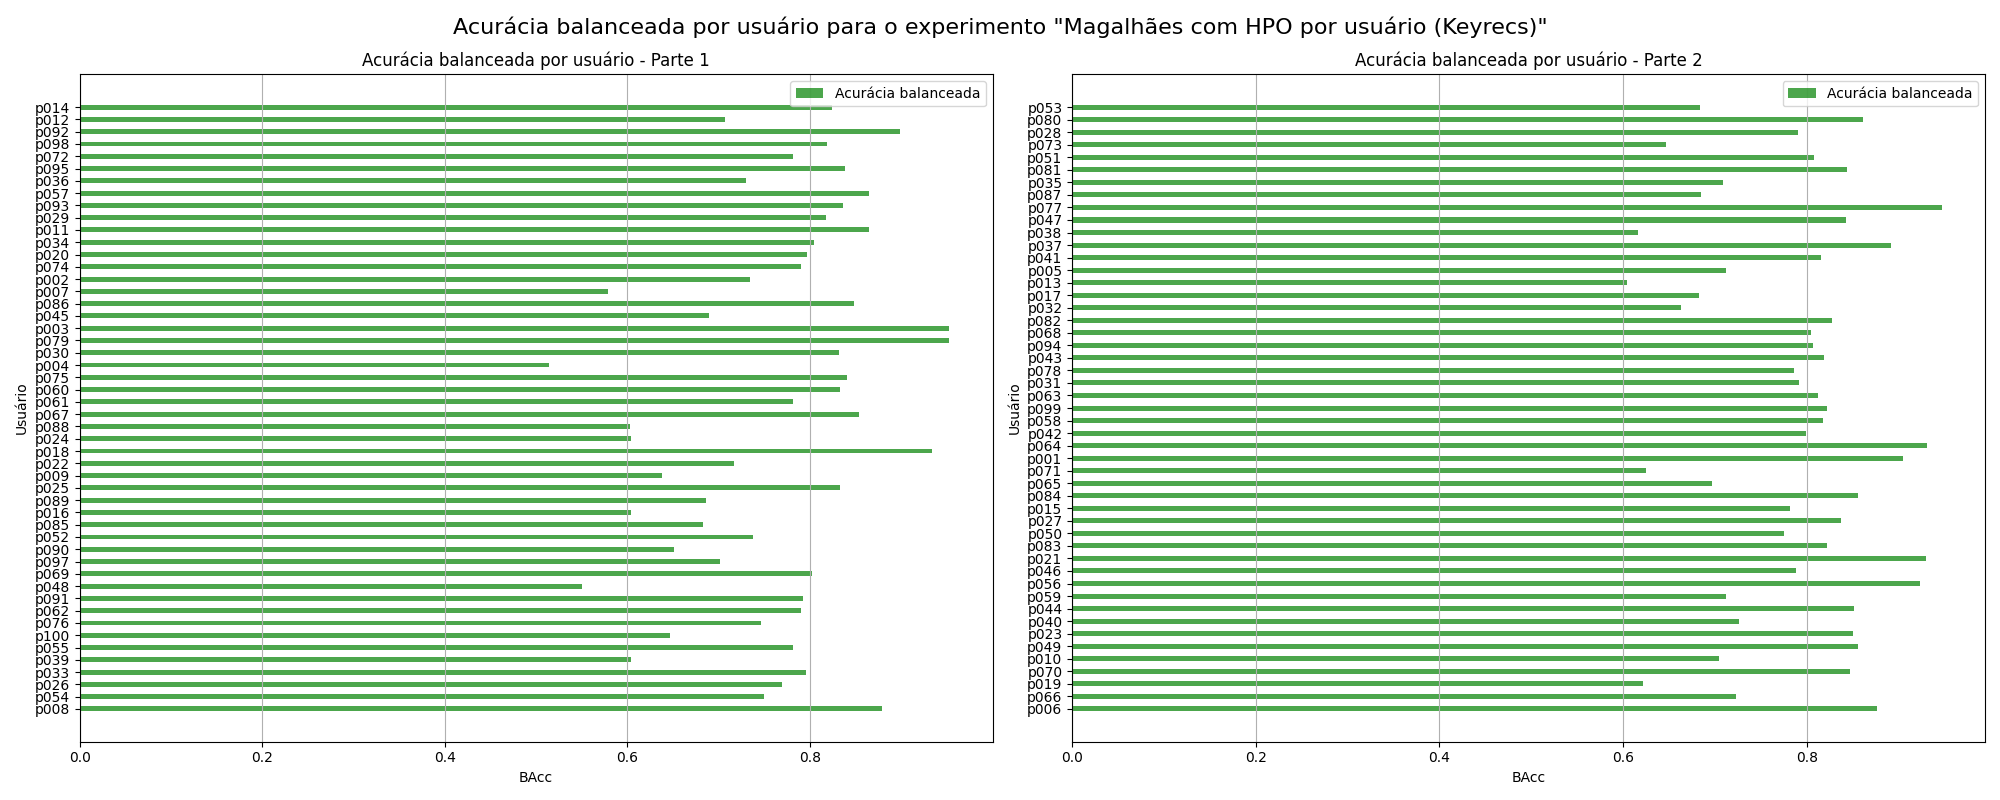
\includegraphics[width=\textwidth]{Magalhães com HPO por usuário (Keyrecs) - BAcc.png}
\end{figure}
\begin{figure}[H]
    \caption{Random Forest com HPO global (CMU) - BAcc}
    \label{fig:Random Forest com HPO global (CMU) - BAcc}
    \centering
    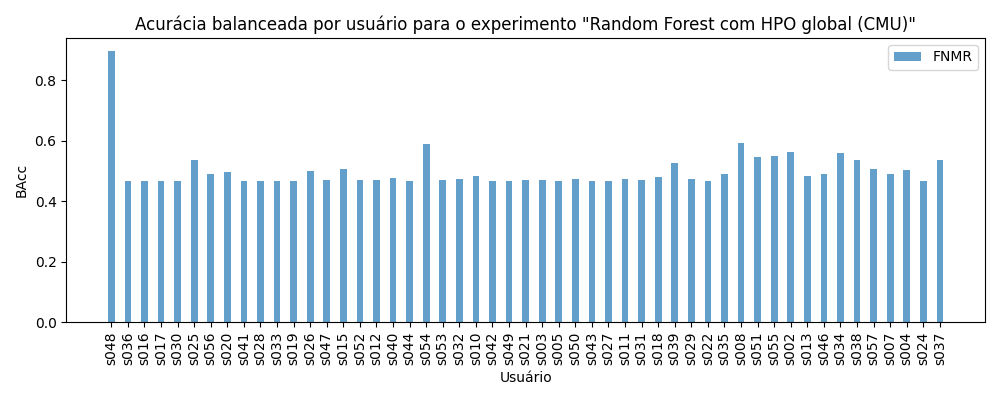
\includegraphics[width=\textwidth]{Random Forest com HPO global (CMU) - BAcc.png}
\end{figure}
\begin{figure}[H]
    \caption{Random Forest com HPO por usuário (CMU) - BAcc}
    \label{fig:Random Forest com HPO por usuário (CMU) - BAcc}
    \centering
    \includegraphics[width=\textwidth]{Random Forest com HPO por usuário (CMU) - BAcc.png}
\end{figure}
\begin{figure}[H]
    \caption{SVM (CMU) - BAcc}
    \label{fig:SVM (CMU) - BAcc}
    \centering
    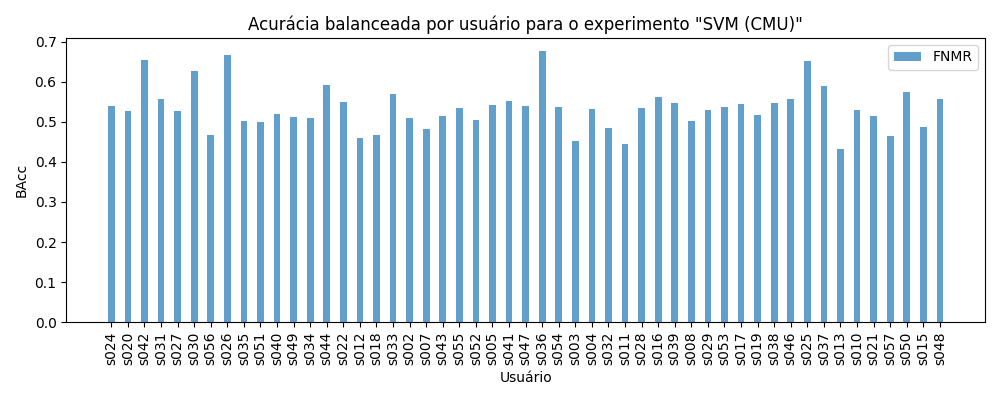
\includegraphics[width=\textwidth]{SVM (CMU) - BAcc.png}
\end{figure}
\begin{figure}[H]
    \caption{SVM (Keyrecs) - BAcc}
    \label{fig:SVM (Keyrecs) - BAcc}
    \centering
    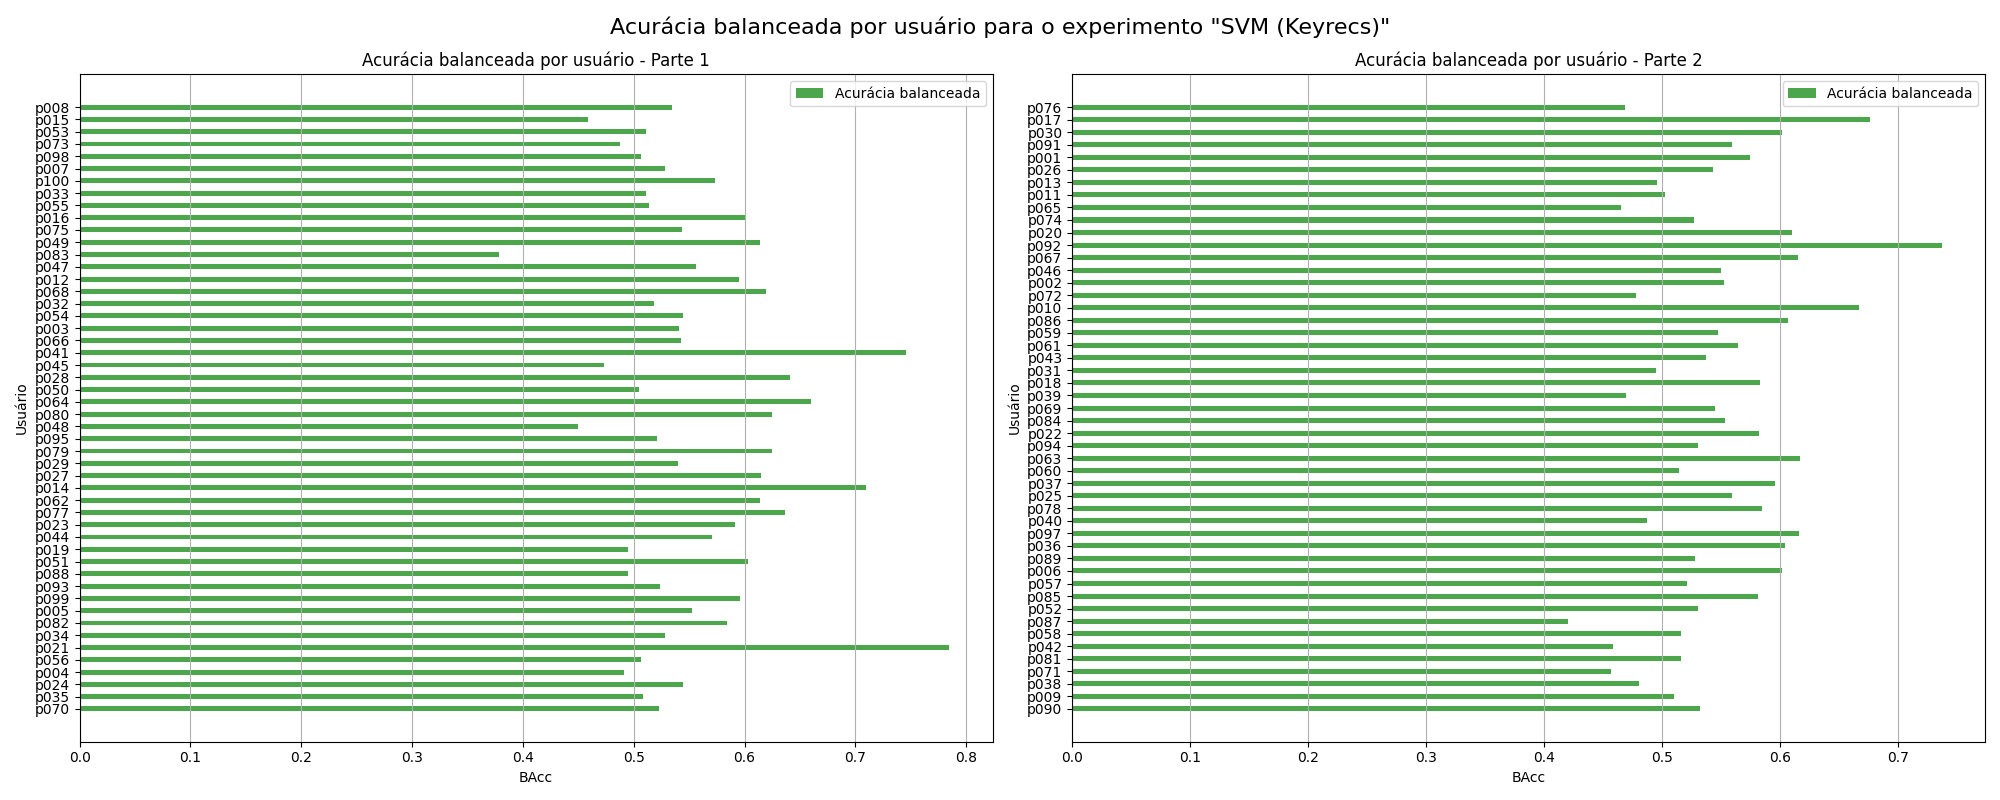
\includegraphics[width=\textwidth]{SVM (Keyrecs) - BAcc.png}
\end{figure}
\begin{figure}[H]
    \caption{SVM com HPO global (CMU) - BAcc}
    \label{fig:SVM com HPO global (CMU) - BAcc}
    \centering
    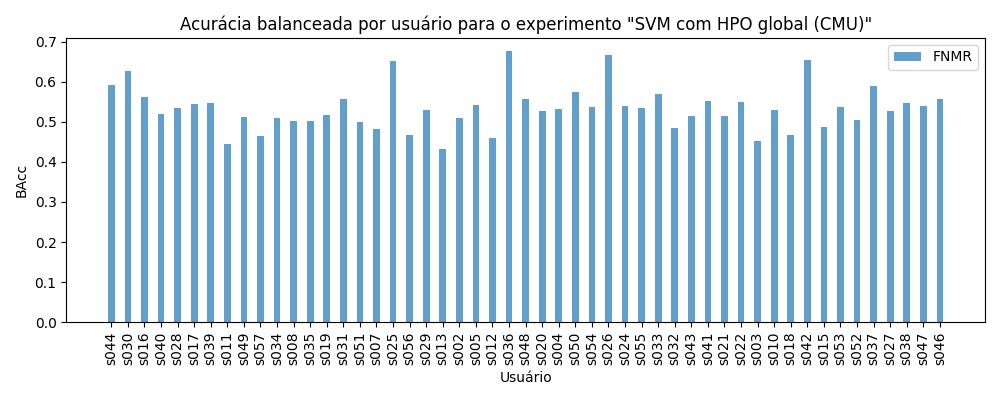
\includegraphics[width=\textwidth]{SVM com HPO global (CMU) - BAcc.png}
\end{figure}
\begin{figure}[H]
    \caption{SVM com HPO global (Keyrecs) - BAcc}
    \label{fig:SVM com HPO global (Keyrecs) - BAcc}
    \centering
    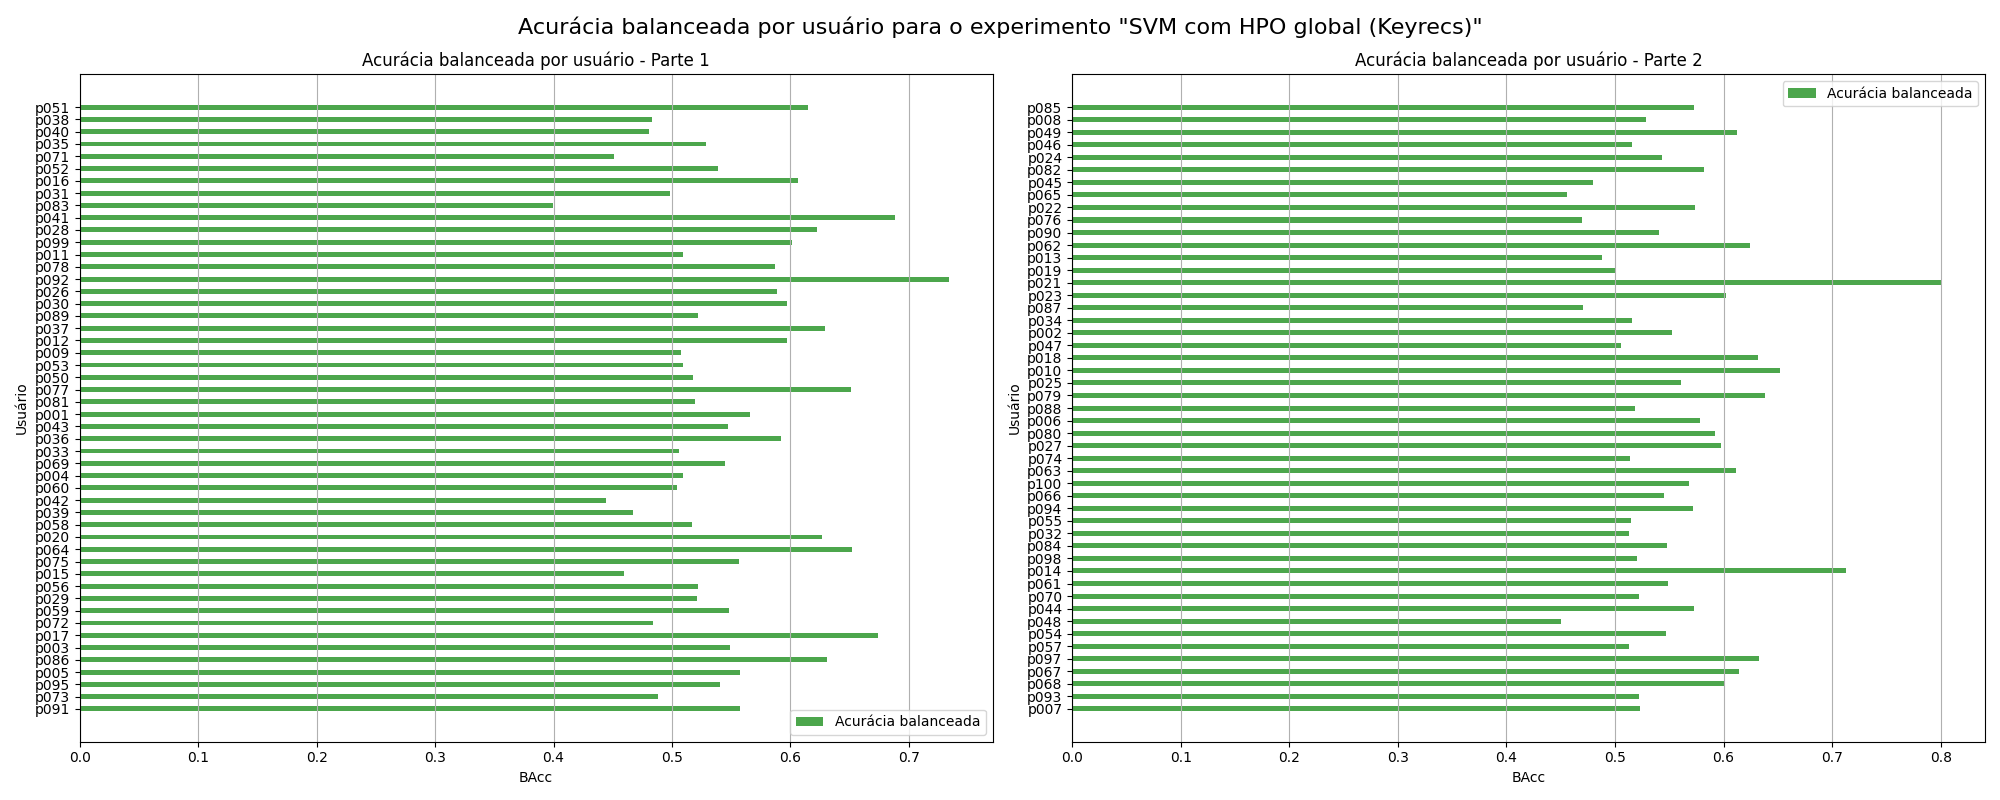
\includegraphics[width=\textwidth]{SVM com HPO global (Keyrecs) - BAcc.png}
\end{figure}
\begin{figure}[H]
    \caption{SVM com HPO por usuário (CMU) - BAcc}
    \label{fig:SVM com HPO por usuário (CMU) - BAcc}
    \centering
    \includegraphics[width=\textwidth]{SVM com HPO por usuário (CMU) - BAcc.png}
\end{figure}
\begin{figure}[H]
    \caption{SVM com HPO por usuário (Keyrecs) - BAcc}
    \label{fig:SVM com HPO por usuário (Keyrecs) - BAcc}
    \centering
    \includegraphics[width=\textwidth]{SVM com HPO por usuário (Keyrecs) - BAcc.png}
\end{figure}